% ============================================================================
% Paper 1 (CLeaR-shaped): "When Can You Trust an Equilibrium Counterfactual?"
% Draft 2026-07-16, branch equilibrium-counterfactuals (local only).
%
% PRE-SUBMISSION TODOs (owner):
%  - STYLE: typeset with the jmlr class in [pmlr] mode (jmlr.cls, jmlrutils.sty,
%    algorithm2e.sty vendored alongside; CLeaR proceedings are PMLR volumes and
%    the per-year CLeaR style is a thin wrapper over this class). When the
%    CLeaR 2027 author kit is released, swap in its wrapper .sty and set the
%    volume/workshop fields it prescribes.
%  - ANONYMIZED: the library is never named and no API identifiers appear
%    anywhere (theory-paper identity + double-blind hygiene + the standing
%    strategy of keeping the library launch separate from the paper wave).
%    Remaining step at submission: attach the anonymized code artifact
%    (in ./artifact, zipped as artifact.zip) referenced in Appendix E.
%  - PAGE BUDGET: main text (through Conclusion) currently ends on p.15 in
%    this format; CLeaR's historical limit is 12pp excluding references and
%    appendices. Trim candidates: Related Work prose, Section 5's diagnostics
%    paragraph, E1 honesty notes (move to Appendix E).
%  - Residual reading checks from the due-diligence report (also flagged in
%    references.bib): Hammond et al. pre-policy section; Mishra--Fox in full;
%    Magnolfi--Roncoroni published ANR treatment; EC 2024--26 proceedings scan;
%    exact CE-complexity citations.
%  - Verify Dogra staff-report number/year.
% ============================================================================
\documentclass[pmlr]{jmlr}
% Class auto-loads: amsmath, amssymb, natbib, graphicx, url, xcolor, hyperref, algorithm2e.

\usepackage{mathtools}
\usepackage{booktabs}
\usepackage{microtype}

% The class predefines theorem/lemma/corollary/proposition/definition/remark/example
% (shared counter, jmlrutils); only `assumption` is missing.
\theorembodyfont{\normalfont}
\newtheorem{assumption}[theorem]{Assumption}
\theorembodyfont{\normalfont\itshape}
% The class's proof environment takes no optional argument; extend it.
\renewenvironment{proof}[1][\proofname]%
  {\par\noindent{\bfseries\upshape #1.\ }}{\jmlrQED}

% --- notation -----------------------------------------------------------------
\newcommand{\R}{\mathbb{R}}
\newcommand{\E}{\mathbb{E}}
\newcommand{\Prob}{\mathbb{P}}
\newcommand{\doop}{\mathrm{do}}
\newcommand{\doeq}[1]{\doop^{\mathrm{eq}}(#1)}
\newcommand{\dolr}[1]{\doop^{\mathrm{lr}}(#1)}
\newcommand{\CCE}{\mathrm{CCE}}
\newcommand{\margin}{\mathrm{margin}}
\newcommand{\gstar}{\gamma^{*}}
\newcommand{\Cid}{\textsc{Identified}}
\newcommand{\Cbd}{\textsc{Bounded}}
\newcommand{\Cem}{\textsc{Empirical}}
\newcommand{\code}[1]{\texttt{#1}}

\jmlrvolume{vvv}
\jmlryear{2027}
\jmlrworkshop{Conference on Causal Learning and Reasoning (under double-blind review)}

\title[When Can You Trust an Equilibrium Counterfactual?]{When Can You Trust an Equilibrium
Counterfactual?\titlebreak A Certified Identification Trichotomy for Interventions on Learning
Systems}
\author{\Name{Anonymous Author(s)} \Email{anonymous@example.com}\\
\addr Anonymized for double-blind review}

\begin{document}
\maketitle

\begin{abstract}
Equilibrium models answer interventional queries by mutilate-and-re-solve --- the
$\doop$-semantics of cyclic structural causal models; learning models answer the same query by
unrolling adaptive dynamics. The two operators can disagree, and the disagreement is the formal
content of a fault line running from the Lucas critique to complexity economics. We make the
question --- \emph{when do the two operators return the same answer?} --- a machine-checkable
identification problem. Our main theorem is a trichotomy for global interventional queries on
populations of adaptive learners: the equilibrium counterfactual is \emph{point-identified}
exactly under expectational stability (E-stability~$\Leftrightarrow$~causal validity of the
$\sigma$-solution, with the sharp learning-rate threshold); it is \emph{set-identified} by a
linear program over the $\varepsilon$-coarse-correlated-equilibrium polytope of the intervened
game, at the regret $\varepsilon_T$ actually measured at the horizon actually run, with no
further assumptions; and otherwise it is \emph{not identified}, but the failure itself is
certifiable, with diagnostics --- including multiplicity, where the honest global object is a
basin-mass mixture no plain SCM can represent. Every condition is computable by instruments we
release as an open-source artifact, each returning a typed certificate, and four experiments
exercise every rung --- including a monetary-policy toy where the \emph{sign} of a policy
conclusion flips between the two semantics exactly where the certificate says not to trust the
equilibrium, and a bistable system with locally correct certificates but a measured global
selection gap.
\end{abstract}

\begin{keywords}
causal identification; cyclic structural causal models; equilibrium; learning in games;
coarse correlated equilibrium; E-stability; certificates
\end{keywords}

% ============================================================================
\section{Introduction}\label{sec:intro}
% ============================================================================

Ask a New-Keynesian toy model what happens to inflation after a unit demand shock under a passive
interest-rate rule, and the equilibrium answer is a \emph{fall} of $8.2$ points: mutilate the
structural equations, re-solve the fixed point, read off the counterfactual. Ask the same
structural equations populated by adaptive learners, and inflation \emph{rises without bound} ---
$+250$ points within thirty learning steps (Section~\ref{sec:e4}). Same model, same intervention,
same query; opposite sign. Under an active rule the two answers agree to machine precision, and
nothing in the equilibrium computation warns which case one is in.

The pattern is old. The Lucas critique \citep{lucas1976econometric} says interventional
predictions computed from an equilibrium description can fail when the underlying adaptation
re-equilibrates; the adaptive-learning program in macroeconomics showed that stability of
learning --- E-stability --- governs whether rational-expectations equilibria are attainable at
all \citep{marcet1989convergence,evans2001learning}; \citet{dogra2024paradoxes} argues the causal
interpretation of equilibrium economics is paradox-ridden precisely because equilibrium models
suppress the adjustment process; complexity economics has long insisted that ``equations'' and
``maps'' are different objects \citep{brock1997rational,pangallo2019best}. On the
causal-inference side, cyclic SCMs give equilibrium counterfactuals an exact semantics
\citep{bongers2021foundations}, the ODE-to-SCM construction says when an SCM abstracts an
underlying dynamical system \citep{mooij2013ordinary,rubenstein2017causal}, and
\citet{blom2019beyond} prove that equilibria depending on initial conditions are what no plain
SCM can represent. What none of these provides is an \emph{identification theory}: exactly when
does the equilibrium $\doop$-operator answer the interventional question posed of the adaptive
system, what can be salvaged when it does not, and a procedure that checks and says so.

This paper provides that theory for two well-delimited classes --- cyclic SCMs with smooth mean
fields, and finite games --- with instruments that make every condition checkable:

\begin{enumerate}
\item \textbf{A bridge theorem (Theorems~\ref{thm:t1} and~\ref{thm:t1prime}).} For linear cyclic
SCMs, point identification of the learning-limit counterfactual by the equilibrium counterfactual
holds \emph{if and only if} the intervened system is E-stable \citep{evans2001learning}, with the
sharp constant-gain threshold $\gstar$ in closed form: \emph{the $\sigma$-solution of the cyclic
SCM is the causally correct description of the learning population exactly on the E-stable
class}. A corollary formalizes the equations-vs-maps gap (naive unrolling demands the strictly
stronger $\rho(B)<1$; divergent map with convergent learners is a nonempty, certifiable regime),
and Theorem~\ref{thm:t1prime} extends both directions to hyperbolic equilibria of smooth systems,
with explicit noise conditions, at the price of basin-local scope.
\item \textbf{An identification trichotomy (Theorem~\ref{thm:main}).} For global interventional
queries posed of learning populations in the two classes, exactly one of three cases holds, each
decidable by a finite computation and mapped to a typed certificate: \emph{point} identification
(\Cid), \emph{set} identification by LP bounds over the $\varepsilon_T$-CCE polytope of the
intervened game at the \emph{measured} realized regret (\Cbd; Theorem~\ref{thm:t2},
assumption-free at every finite horizon), and \emph{certified non-identification} (\Cem) with
diagnostics.
\item \textbf{Certified failure rather than silent failure.} In the non-identified case the
instruments report \emph{why}: a negative margin no learning rate can rescue; abstention in
place of a vacuous bound; or multiplicity, where the global object is a basin-mass mixture ---
the causal-constraint-model caveat of \citet{blom2019beyond} operationalized and, in our
experiments, \emph{measured}.
\item \textbf{Instruments and evidence.} Every condition is computed by exact, dependency-free
instruments released as an open-source artifact (stability-margin diagnostic and damped
comparator for cyclic SCMs; CCE polytope, LP bounds, measured-regret certificates, and dual
sensitivities for games); four experiments exercise every rung of the resulting ladder
(Section~\ref{sec:experiments}).
\end{enumerate}

\paragraph{What this paper is not.} The mathematical ingredients are standard ---
stochastic approximation on one side, LP duality over equilibrium polytopes on the other --- and
Theorem~\ref{thm:t2} is a rearrangement of the definition of regret. The contribution is the
synthesis: the two-semantics framing, the bridge, the trichotomy, and the instruments plus
experiments demonstrating the ladder end to end. We state each theorem's provenance next to it
and flag every place where our experimental claims stop short (Section~\ref{sec:limitations}).

% ============================================================================
\section{Two \texorpdfstring{$\doop$}{do} semantics for one query}\label{sec:setup}
% ============================================================================

\subsection{Equilibrium \texorpdfstring{$\doop$}{do}: cyclic SCMs}\label{sec:eqdo}

A cyclic SCM over endogenous $x \in \R^n$ and exogenous $u$ specifies structural equations
$x_i = f_i(x_{\mathrm{pa}(i)}, u_i)$ whose dependency graph may contain cycles; its solutions
are the fixed points $x = f(x, u)$, given interventional semantics by the solution-function
($\sigma$-solution) theory of \citet{bongers2021foundations}. The \textbf{equilibrium $\doop$}
is mutilate-and-re-solve: replace the targeted equations, then solve the intervened fixed-point
problem. Throughout, our exact linear class is
\begin{equation}\label{eq:linear-scm}
x = Bx + u, \qquad
\doop(x_i{=}\xi):\ \text{zero row } i \text{ of } B,\ \text{pin } u_i = \xi,
\end{equation}
with intervened pair $(B_{\doop}, u_{\doop})$ and, whenever $I - B_{\doop}$ is invertible, the
unique equilibrium counterfactual
\begin{equation}\label{eq:xstar}
x^* \;=\; (I - B_{\doop})^{-1}\, \E[u_{\doop}].
\end{equation}
We write $\doeq{\cdot}$ for this operator; for finite games (Section~\ref{sec:t2}) the
equilibrium object is a set rather than a point, with the correlated-equilibrium polytope
playing the role of $(I-B)^{-1}$.

\subsection{Learning \texorpdfstring{$\doop$}{do}: adaptive dynamics}\label{sec:lrdo}

Populated instead by agents who adapt rather than solve fixed points, the same equations define
a process: impose the same mutilation on the \emph{process} and unroll,
\begin{equation}\label{eq:sa}
x_{k+1} \;=\; x_k + \gamma_k \bigl( f_{\doop}(x_k) - x_k + M_{k+1} \bigr),
\end{equation}
where $\gamma_k$ is a gain sequence and $M_{k+1}$ is martingale-difference noise. Constant gain
$\gamma_k \equiv \gamma \in (0,1]$ is the Euler discretization of the \textbf{mean dynamics}
\begin{equation}\label{eq:ode}
\dot{x} \;=\; F_{\doop}(x) \;\coloneqq\; f_{\doop}(x) - x,
\end{equation}
and decreasing gain ($\sum_k \gamma_k = \infty$, $\sum_k \gamma_k^2 < \infty$) is Robbins--Monro
stochastic approximation \citep{robbins1951stochastic}, the regime of least-squares learning in
macroeconomics \citep{marcet1989convergence,evans2001learning}. Equation~\eqref{eq:ode} is the
E-stability ODE of \citet{evans2001learning} in mean-dynamics form: $f_{\doop}$ is the
temporary-equilibrium map from expectations to realized outcomes, and E-stability of an
equilibrium $x^*$ is local asymptotic stability of $x^*$ under \eqref{eq:ode}. The
\textbf{learning $\doop$}, written $\dolr{\cdot}$, is the long-run behavior of \eqref{eq:sa}: its
almost-sure limit when one exists, and its time-averaged play otherwise.

Two spectral quantities decide everything in the linear class. With
$\nu_i = \lambda_i(B_{\doop}) - 1$ the eigenvalues of the mean-dynamics Jacobian
$B_{\doop} - I$,
\begin{equation}\label{eq:margin}
\margin(B_{\doop}) \;=\; 1 - \max_i \operatorname{Re} \lambda_i(B_{\doop}),
\qquad
\gstar \;=\; \min_i \frac{-2\operatorname{Re}\nu_i}{|\nu_i|^2},
\end{equation}
the \emph{stability margin} (positive iff $B_{\doop}-I$ is Hurwitz) and the \emph{maximal stable
learning rate} (the sharp constant-gain threshold, Lemma~\ref{lem:gain}).

\subsection{Queries and certificates}\label{sec:queries}

A \emph{query} is the long-run population value $Q = \E_\mu[h]$ of a functional $h$ under the
intervention, where $\mu$ is the population's long-run occupation law. We distinguish
\emph{global} queries --- the population's long-run behavior, full stop --- from
\emph{basin-local} queries conditioned on initialization within the basin of a stable solution;
Section~\ref{sec:e7} measures a system where every basin-local query is point-identified while
the global query is not. The equilibrium counterfactual \emph{point-identifies} the query when
$\dolr{\cdot}$ exists as a point and equals $\doeq{\cdot}$; \emph{set-identifies} it when a
computable set provably contains the realized value; and \emph{fails} otherwise.
\label{sec:certificates}%
Every instrument returns a typed certificate: a rung in $\{\Cid, \Cbd, \Cem\}$, a claim, a
machine-checkable \emph{witness} (spectra, LP values, dual multipliers, measured regrets), and
\emph{hedges} --- what blocked a stronger rung and, when possible, the action that would unblock
it. The rung ordering is a soundness contract: \Cid{} only under a proof of point
identification, \Cbd{} only under a proof of containment, everything else degrading to \Cem{}
with diagnostics rather than fabricating a bound. The $\doop$-comparator for cyclic SCMs and the
game certifier for finite games implement the ladder in Table~\ref{tab:ladder}.

% ============================================================================
\section{Point identification: E-stability is causal validity}\label{sec:t1}
% ============================================================================

\begin{lemma}[gain window]\label{lem:gain}
Let $\nu \in \mathbb{C}$. If $\operatorname{Re}\nu < 0$ then $|1 + \gamma\nu| < 1$ iff
$0 < \gamma < -2\operatorname{Re}\nu / |\nu|^2$. If $\operatorname{Re}\nu \geq 0$ then
$|1 + \gamma\nu| \geq 1$ for every $\gamma > 0$.
\end{lemma}
\begin{proof}
$|1+\gamma\nu|^2 - 1 = \gamma\,(2\operatorname{Re}\nu + \gamma |\nu|^2)$, which is negative iff
$\gamma < -2\operatorname{Re}\nu/|\nu|^2$, a positive threshold iff $\operatorname{Re}\nu < 0$;
if $\operatorname{Re}\nu \geq 0$ the right factor is nonnegative for all $\gamma>0$.
\end{proof}

\begin{theorem}[T1: point identification $\Leftrightarrow$ E-stability; linear class]\label{thm:t1}
Let $x = Bx + u$ be a linear cyclic SCM with intervened pair $(B_{\doop}, u_{\doop})$,
$I - B_{\doop}$ invertible, $x^*$ as in \eqref{eq:xstar}, and learning dynamics \eqref{eq:sa}
with $f_{\doop}(x) = B_{\doop} x + u_{\doop,k}$, $\E[u_{\doop,k}] = \E[u_{\doop}]$, and noise
with bounded conditional second moments. The following are equivalent:
\begin{enumerate}
\item[(1)] \emph{E-stability:} $\margin(B_{\doop}) > 0$, i.e.\ $B_{\doop} - I$ is Hurwitz;
\item[(2)] \emph{constant gain:} for every $\gamma \in (0, \gstar)$ the mean iteration converges
to $x^*$ from every initial condition, and the stochastic iterates satisfy
$\limsup_k \E\|x_k - x^*\|^2 = O(\gamma)$;
\item[(3)] \emph{decreasing gain:} Robbins--Monro learning converges to $x^*$ almost surely
(boundedness of the iterates has probability one under (1) for the linear recursion).
\end{enumerate}
Under any of these, $\dolr{\cdot} = \doeq{\cdot}$: the $\sigma$-solution of the intervened cyclic
SCM is the causally correct description of the learning population's interventional behavior.
Conversely, if $\margin(B_{\doop}) < 0$: for every $\gamma > 0$ the mean iteration diverges from
all initial conditions outside a proper subspace, and with noise nondegenerate in the unstable
directions, decreasing-gain learning converges to $x^*$ with probability zero. The learning-limit
$\doop$ then does not exist as a point, and the equilibrium prediction has no dynamical
counterpart.
\end{theorem}

\begin{proof}[Proof (algebraic part; stochastic parts in Appendix~\ref{app:t1})]
The mean iteration is $x_{k+1} = M_\gamma x_k + \gamma \E[u_{\doop}]$ with
$M_\gamma = I + \gamma(B_{\doop} - I)$, whose fixed point is $x^*$ for \emph{every} $\gamma$ ---
damping never moves the equilibrium, only the convergence class. Its eigenvalues are
$1 + \gamma\nu_i$; by Lemma~\ref{lem:gain}, $\rho(M_\gamma) < 1$ for all $\gamma \in (0,\gstar)$
iff every $\operatorname{Re}\nu_i < 0$, i.e.\ iff (1), and $\gstar$ in \eqref{eq:margin} is sharp.
If some $\operatorname{Re}\nu_i > 0$ then $|1 + \gamma\nu_i| > 1$ for all $\gamma > 0$, giving
divergence along that eigenspace. The noise bound in (2), the ODE-method equivalence
(1)$\Leftrightarrow$(3) \citep{ljung1977analysis,kushner2003stochastic,benaim1999dynamics}, and
the probability-zero converse \citep{pemantle1990nonconvergence,brandiere1996algorithmes} are in
Appendix~\ref{app:t1}.
\end{proof}

Theorem~\ref{thm:t1} is a bridge, and we claim it as such: each direction is classical in its
home literature, but the equivalence has, to our knowledge, never been stated as a statement
about the validity of SCM $\doop$-semantics --- ``E-stability'' becomes ``the $\sigma$-solution
is the causally correct object,'' a sentence neither literature could previously parse.

\begin{corollary}[naive unrolling is a strictly stronger demand]\label{cor:maps}
The literal period-$1$ unrolling $x_{k+1} = B_{\doop} x_k + u$ converges iff
$\rho(B_{\doop}) < 1$. Since $\rho(B) < 1 \Rightarrow \max_i \operatorname{Re}\lambda_i(B) < 1$
but not conversely, the regime $\{\rho(B_{\doop}) \geq 1,\ \margin(B_{\doop}) > 0\}$ is nonempty
(e.g.\ $B = [\,-2\,]$: $\rho = 2$, $\margin = 3$): the map diverges while every sufficiently
damped adaptive population converges to the equilibrium counterfactual --- the formal content of
the equations-vs-maps gap in the linear class, certified by the comparator at any
$\gamma < \gstar$.
\end{corollary}

\subsection{The nonlinear local statement}\label{sec:t1prime}

Let $F = f - \mathrm{id}$ with $f \in C^1$, and let $x^*$ be a \emph{hyperbolic} zero of $F$ (no
eigenvalue of $J = DF(x^*)$ on the imaginary axis); assumptions (A1)--(A4) are stated in
Appendix~\ref{app:t1prime}.

\begin{theorem}[T1$'$: hyperbolic local version]\label{thm:t1prime}
Under (A1)--(A3):
\begin{enumerate}
\item[(i)] If $J$ is Hurwitz, then for every $\gamma \in (0, \gstar(J))$ (the formula in
\eqref{eq:margin} evaluated on the spectrum of $J$) the constant-gain iteration is locally
exponentially stable at $x^*$ with asymptotic mean-square error $O(\gamma)$, and decreasing-gain
iterates converge to $x^*$ almost surely on the event of remaining in a compact subset of the
basin of attraction of $x^*$. Hence $\dolr{\cdot} = \doeq{\cdot}$ \emph{locally, on the basin of}
$x^*$.
\item[(ii)] If $J$ has an eigenvalue with positive real part, then under the additional
excitation condition (A4), $\Prob(x_k \to x^*) = 0$: the equilibrium counterfactual at $x^*$ has
no learning-limit counterpart.
\end{enumerate}
\end{theorem}

\begin{proof}[Proof sketch]
Hyperbolicity reduces (i) to the linear case via Hartman--Grobman plus the SA limit-set theorem
\citep{kushner2003stochastic,benaim1999dynamics,borkar2008stochastic}; (ii) is
nonconvergence-to-unstable-points
\citep{pemantle1990nonconvergence,brandiere1996algorithmes}. Full proof with explicit noise
conditions: Appendix~\ref{app:t1prime}.
\end{proof}

\begin{remark}[the basin qualifier binds]\label{rem:selection}
T1$'$ is local by nature. With \emph{multiple} stable $\sigma$-solutions, every basin-local
certificate can be simultaneously correct while the global interventional outcome is a
\emph{basin-mass mixture} across them --- and interventions move both the solutions and the
basin boundaries. \citet{blom2019beyond} prove that equilibria depending on initial conditions
are exactly what plain SCM semantics cannot represent; equilibrium selection by learning is that
phenomenon, not an analogy to it. Section~\ref{sec:e7} measures the resulting gap; hence the
trichotomy below classifies global queries and treats multiplicity as certified
non-identification.
\end{remark}

% ============================================================================
\section{Set identification: the measured-regret CCE rung}\label{sec:t2}
% ============================================================================

The second exact class is finite games, where the equilibrium object is a set and the honest
counterpart of \eqref{eq:xstar} is a polytope. Let $G$ be a finite game with agents $N$, action
sets $A_i$, and utilities $u_i$; an intervention pins the actions of a subset of agents,
inducing $G_{\doop}$ (profiles restricted to the consistent ones, no-deviation constraints only
for free agents) --- in the causal-games taxonomy, pre-policy for the free agents, whose play
re-adapts, and post-policy for the pinned ones \citep{hammond2023reasoning,mishra2024causal}. For $\varepsilon = (\varepsilon_i)_{i}$, the
$\varepsilon$-coarse-correlated-equilibrium polytope is
\begin{equation}\label{eq:cce}
\CCE_{\varepsilon}(G_{\doop}) \;=\; \Bigl\{ \mu \in \Delta(\text{profiles}) \;:\;
\E_{\mu}\bigl[u_i(a_i', s_{-i}) - u_i(s)\bigr] \leq \varepsilon_i
\ \ \forall i \text{ free},\ \forall a_i' \in A_i \Bigr\}.
\end{equation}
A population plays $T$ rounds of $G_{\doop}$, producing the empirical joint distribution $\mu_T$;
agent $i$'s \emph{realized regret}
$\varepsilon_T(i) = \max_{a_i'} \frac{1}{T}\sum_{t=1}^{T}
[\,u_i(a_i', s_{-i,t}) - u_i(s_t)\,]$, clipped at zero, is computable from the trajectory log.

\begin{theorem}[T2: finite-time containment, assumption-free]\label{thm:t2}
For every horizon $T$ and every profile functional $h$,
\[
\E_{\mu_T}[h] \;\in\; \Bigl[\, \min_{\mu} \E_\mu[h],\ \max_{\mu} \E_\mu[h]
\Bigr] \quad \text{over } \mu \in \CCE_{\varepsilon_T}(G_{\doop}),
\]
where $\varepsilon_T$ is the vector of measured realized regrets. Both endpoints are linear
programs over a polytope contained in the simplex.
\end{theorem}
\begin{proof}
$\mu_T \in \CCE_{\varepsilon_T}(G_{\doop})$ is the definition of realized regret rearranged: the
expected deviation gain of switching to a fixed $a_i'$ under $\mu_T$ \emph{is} the time-averaged
realized gain, which is at most $\varepsilon_T(i)$ by construction. Containment of
$\E_{\mu_T}[h]$ between the min and max over the feasible set is then immediate.
\end{proof}

Theorem~\ref{thm:t2} is definitionally true, and we present it as such: the ex post, finite-time
character of measured-regret sets is folklore in the full-feedback case --- the rationalizable
set of \citet{nekipelov2015econometrics} already holds for the realized play, as
\citet{hartline2026economics} emphasizes --- and the containment step is textbook. Its role here
is to be the \emph{set-identification rung of the trichotomy}: binding at the horizon actually
run, for whatever the learners actually did, abstaining when vacuous, and horizon-uniform
(deterministic given the log at every $T$). Three corollaries complete the rung.

\begin{corollary}[asymptotic route]\label{cor:asymptotic}
If the population is no-regret ($\varepsilon_T \to 0$;
\citealp{foster1997calibrated,hart2000simple}), every limit point of $\{\mu_T\}$ lies in
$\CCE_0(G_{\doop})$ and the $\varepsilon_T$-bounds converge to the exact-CCE bounds (the LP
value is Lipschitz in the right-hand side): the classical statement is the $\varepsilon \to 0$
limit of the certified one.
\end{corollary}

\begin{corollary}[degeneracy: when the equilibrium point prediction is safe]\label{cor:degeneracy}
The equilibrium point prediction of $h$ is valid for every no-regret population iff
$h$ is constant over $\CCE_0(G_{\doop})$ (LP width $0$) --- a checkable condition, certified
\Cid. Example: every CCE of a two-player zero-sum game achieves the value, so value functionals
are point-identified; generic anti-coordination games are not.
\end{corollary}

\begin{corollary}[$\varepsilon$-sensitivity from LP duals]\label{cor:duals}
Each endpoint is a concave (max side) or convex (min side) piecewise-linear function of
$\varepsilon$, with one-sided derivative at the measured $\varepsilon_T$ equal to the sum of the
optimal dual multipliers on the perturbed constraints --- reported in the certificate witness.
It prices the marginal tightness bought by running the population longer; an interval that is
wide while its sensitivity is tiny is \emph{structurally} loose (the game), not statistically
loose (the learners) --- a distinction no asymptotic statement makes.
\end{corollary}

\begin{remark}[width is the operational content of ``equilibrium'']\label{rem:width}
$\mathrm{width}(h, \doop) = \max - \min$ over $\CCE_0(G_{\doop})$ measures how much predictive
content equilibrium analysis has under that intervention: zero is point identification; the
full payoff range is none --- and the certificate \emph{abstains} rather than report a vacuous
interval.
\end{remark}

\begin{remark}[scope: the stage-game polytope]\label{rem:scope}
$\CCE_{\varepsilon}(G_{\doop})$ is the \emph{stage-game} polytope. Populations with
history-dependent strategies and intertemporal objectives --- empirically, the
value-bootstrapping learners of the algorithmic-collusion literature
\citep{calvano2020artificial} --- can sustain time-averages outside it. Theorem~\ref{thm:t2} is
not violated: such populations are \emph{detected, not missed} --- their measured
$\varepsilon_T$ stays bounded away from zero and the certificate inflates or abstains. Mapping
which families escape is companion work; the trichotomy only needs that containment itself is
unconditional.
\end{remark}

\paragraph{Provenance.} Every atomic ingredient of this section exists in some form, and the
delta is exactly the conjunction of four choices no adjacent work makes --- $\varepsilon$ from
\emph{measured} play, containment on the \emph{intervened} game, abstention, dual prices ---
plus the trichotomy and the width reading; Section~\ref{sec:related} states the claim against
each neighbor, nearest of which is \citet{lomys2025estimation}. The LP lives in joint-profile
space (exponential in the number of players; hardness results exist for succinct games,
\citealp{papadimitriou2008computing}), so exact bounds are for small games; sampled and relaxed
bounds are the scale path.

% ============================================================================
\section{The main theorem: an identification trichotomy}\label{sec:main}
% ============================================================================

We now assemble the pieces. The theorem classifies \emph{global} queries; per
Remark~\ref{rem:selection}, point identification requires \emph{global} uniqueness of the stable
$\sigma$-solution, and everything outside the stated regularity routes to diagnostics.

\begin{assumption}[regularity for the nonlinear SCM class]\label{ass:R}
The intervened mean field $F_{\doop} = f_{\doop} - \mathrm{id}$ is $C^1$ with (R1) finitely many
zeros, all hyperbolic; (R2) SA iterates remain in a compact set almost surely (dissipativity);
(R3) the chain-recurrent set of the mean flow consists of its zeros only (no cycles or chaotic
sets). (R1)--(R3) hold automatically in the linear class with $\margin \neq 0$; (R3) is automatic for
scalar systems with hyperbolic zeros. (R2)--(R3) are not decidable a priori: the instruments
guard them at runtime (divergence detection, largest-Lyapunov estimate), and their failure
routes to case~3 below.
\end{assumption}

\begin{theorem}[identification trichotomy for learning populations]\label{thm:main}
Let $Q = \E_\mu[h]$ be a global interventional query posed of a population of adaptive
learners \eqref{eq:sa}, where the intervened system is (a) a linear cyclic SCM, (b) a smooth mean
field satisfying Assumption~\ref{ass:R}, or (c) a finite game played over $T$ rounds with
measured realized regrets $\varepsilon_T$. Then exactly one of the following holds, each
condition computable by a shipped instrument, and the corresponding certificate is warranted:
\begin{enumerate}
\item[\textbf{1.}] \textbf{Point (\Cid).} Either (i) the intervened system \textup{(a)/(b)} has a
\emph{globally unique} stable $\sigma$-solution $x^*$ with $\margin > 0$ (Hurwitz Jacobian):
then for every $\gamma \in (0, \gstar)$, and almost surely under decreasing gain, the learning
$\doop$ equals the equilibrium $\doop$ at $x^*$ (Theorems~\ref{thm:t1} and~\ref{thm:t1prime});
or (ii) the system is a finite game and $h$ is constant over $\CCE_0(G_{\doop})$ (LP width
$\leq$ tol): the equilibrium point prediction holds for every no-regret population
(Corollary~\ref{cor:degeneracy}).
\item[\textbf{2.}] \textbf{Set (\Cbd).} The system is a finite game with LP width $>$ tol and a
nonvacuous interval at the measured $\varepsilon_T$: the realized time-average of $h$ lies
in the LP interval over $\CCE_{\varepsilon_T}(G_{\doop})$, with no further assumptions
(Theorem~\ref{thm:t2}), and the reported dual multipliers price the interval's growth per unit
of additional regret (Corollary~\ref{cor:duals}).
\item[\textbf{3.}] \textbf{None (\Cem, hedged with diagnostics).} One of: every $\sigma$-solution
has unstable mean dynamics ($\margin < 0$ at each; no admissible gain rescues ---
Theorem~\ref{thm:t1} converse); Assumption~\ref{ass:R} fails at runtime (divergence, cycles, or a
positive Lyapunov estimate); the $\varepsilon_T$-interval is vacuous (abstention;
Remark~\ref{rem:width}); or the intervened system has \emph{multiple} stable $\sigma$-solutions,
so the global learning outcome is a basin-mass mixture over them --- an object plain SCM
semantics cannot represent \citep{blom2019beyond} --- reported as a selection hedge (each
stable $\sigma$-solution still carries a correct \emph{basin-local} case-1 certificate; the
trichotomy classifies the global query).
\end{enumerate}
\end{theorem}

\begin{proof}[Proof sketch (details in Appendix~\ref{app:main})]
In classes (a)/(b), enumerate the $\sigma$-solutions (finitely many by (R1)) and count the
stable ones: zero (or (R) failing) $\to$ case~3; exactly one $\to$ case~1(i) via
Theorem~\ref{thm:t1} (globality is automatic in (a); in (b) it follows from (R2)--(R3) plus the
limit-set and nonconvergence theorems); two or more $\to$ case~3 (multiplicity). In class (c):
width $\leq$ tol $\to$ case~1(ii); else a nonvacuous measured-$\varepsilon_T$ interval $\to$
case~2, vacuous $\to$ case~3. Exhaustiveness and exclusivity are by construction (1(i) requires
global uniqueness, which case~3's multiplicity clause negates; 1(ii) and 2 split on width), and
each condition is a finite computation given the enumerated solutions.
\end{proof}

\begin{table}[t]
\centering
\small
\begin{tabular}{lll}
\toprule
condition & instrument & certificate \\
\midrule
$\rho(B_{\doop}) < 1$, gap $\leq$ tol & comparator (naive unrolling) & \Cid \\
$\margin > 0$, $\gamma < \gstar$, gap $\leq$ tol & comparator (damped, T1) & \Cid \\
$\margin > 0$ but naive unrolling diverges & comparator hedge + $\gstar$ & \Cem{} (actionable) \\
$h$ constant over $\CCE_0(G_{\doop})$ & game certifier (T2 degeneracy) & \Cid \\
no-regret assumed or $\varepsilon_T$ measured & game certifier (T2) & \Cbd \\
$\varepsilon_T$-interval vacuous & game certifier & \Cem{} (abstention) \\
$\margin < 0$ at every $\sigma$-solution & comparator hedge (no rescuing $\gamma$) & \Cem{} (certified failure) \\
$I - B_{\doop}$ singular / $\margin \approx 0$ / multiplicity & typed refusal + selection hedge & \Cem{} (selection / CCM caveat) \\
\bottomrule
\end{tabular}
\caption{The certificate ladder: every rung of Theorem~\ref{thm:main}, its instrument, and the
certificate warranted. ``Actionable'' hedges name the re-run that would upgrade the rung; the
last row is a typed refusal to fabricate a solution.}
\label{tab:ladder}
\end{table}

\paragraph{Certified failure, not silent failure.} Case~3 is where most of the practical value
lies, because it is the case existing practice silently mislabels. The instruments report: with
$\margin < 0$, the divergence rate and the proof that no learning rate rescues it; with
$\rho(B_{\doop}) \geq 1$ but $\margin > 0$, the actionable hedge of Corollary~\ref{cor:maps};
with cycles or chaos, a largest-Lyapunov diagnostic (time-averaged play of a finite-game
population still satisfies Theorem~\ref{thm:t2}); with multiplicity or singularity, a typed
refusal carrying all stable solutions and ensemble basin masses (Section~\ref{sec:e7}). The
ladder is \citet{dash2005restructuring}'s warning --- manipulating the equilibrated model
misleads --- made operational.

% ============================================================================
\section{Experiments}\label{sec:experiments}
% ============================================================================

Four experiments exercise every rung of Table~\ref{tab:ladder}; all numbers are outputs of the
released scripts with fixed seeds (Appendix~\ref{app:exp}), and every LP value carries an
independent weak-duality certificate (slack $\sim 10^{-14}$).

\subsection{E1: the certificate ladder on the canonical stage}\label{sec:e1}

The cobweb market --- demand $D(p) = a - dp$, supply $S(p^e) = c + s p^e$ under naive
expectations, per-unit tax $\doop(\tau{=}1)$ --- is the oldest stage for
equilibrium-vs-dynamics questions \citep{nerlove1958adaptive,hommes1994dynamics};
Table~\ref{tab:e1} runs one market through four regimes.

\begin{table}[t]
\centering
\footnotesize
\begin{tabular}{lll}
\toprule
regime & certificate & key witness values \\
\midrule
A: $s/d = 0.5$, naive & \Cid & gap $8.9 \times 10^{-16}$; $p^* = 6.3333$ \\
B: $s/d = 1.5$, naive & \Cem{} (actionable) & $\rho = 1.225$ diverges; $\margin = +1.0$; hedge $\gstar = 0.8$ \\
B: $s/d = 1.5$, $\gamma = 0.4$ & \Cid & gap $0$; $p^* = 4.2000$ \\
C: trend $b = 1.2$ & \Cem{} (certified failure) & $\margin = -0.095$; $\gstar = 0$: no gain rescues \\
D: nonlinear supply, gain $0.14$ & \Cem{} (hedge: $\gamma > \gstar = 0.073$) & Lyapunov $+0.222$; $f'(p^*) = -26.3$ \\
\bottomrule
\end{tabular}
\caption{E1: one market, four regimes, the full ladder. Regime B is
Corollary~\ref{cor:maps} live: the naive cobweb oscillation diverges while the margin is
positive, the hedge names $\gstar$, and the damped re-run certifies \Cid{} --- Nerlove's
adaptive-expectations rescue, certified. Regime C is the certified-failure rung. Regime D is
chaotic (positive Lyapunov exponent).}
\label{tab:e1}
\end{table}

Regime D's chaos enters through the adaptive gain itself (a monotone naive-expectations cobweb
map admits only fixed points and 2-cycles; \citealp{hommes1994dynamics}): the device that
rescues regime B produces chaos in the nonlinear class --- two \Cem{} hedges, one instrument
(further honesty note in Appendix~\ref{app:exp}).

\subsection{E2: non-convergent learning and the \Cbd{} rung}\label{sec:e2}

The perturbed rock--paper--scissors of \citet{sato2002chaos} (tie payoffs $\epsilon_X = 0.5$,
$\epsilon_Y = -0.1$) is the canonical game in which learning fails to converge to Nash. We tax
$X$'s first action ($\tau = 0.3$), build $G_{\doop}$ explicitly, and run a Hedge population for
$T = 200{,}000$ rounds. The Nash point prediction of $X$'s payoff is $0.0667$; the realized
time-average is $0.1034$, a miss of $0.037$. The measured regret is $\varepsilon_T = 0.0021$ and
the measured-$\varepsilon$ interval $[0.0646,\ 0.3120]$ contains the realized value, as
Theorem~\ref{thm:t2} guarantees. Both readings are honest: the certificate catches what Nash
misses, and the width ($0.24$ against a payoff range $\approx 2.3$) \emph{is} the finding ---
the measured predictive content of ``equilibrium'' here (Remark~\ref{rem:width}). We write
``non-convergent learning,'' not chaos: \citet{sato2002chaos} prove chaos for replicator
families, and we did not verify a positive Lyapunov exponent for this Hedge configuration.

\subsection{E4: the certified policy sign flip}\label{sec:e4}

\begin{figure}[t]
\centering
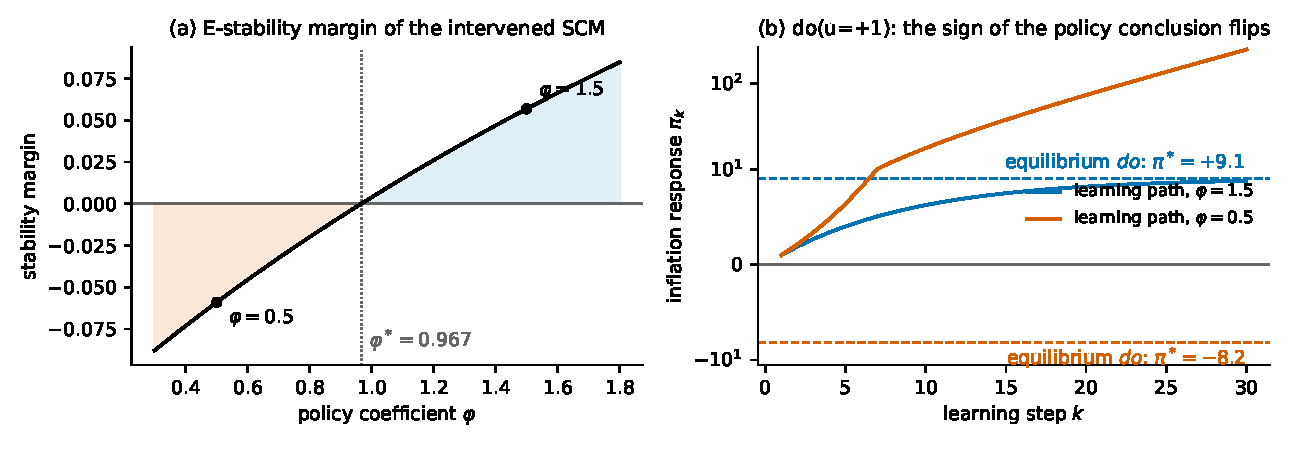
\includegraphics[width=0.82\textwidth]{figs/fig_e4.pdf}
\caption{E4. Left: stability margin of the intervened SCM vs the policy coefficient $\varphi$,
crossing zero at $\varphi^* = 0.9667$. Right: under $\doop(u{=}{+}1)$, learning paths vs the
equilibrium predictions (dashed): at $\varphi = 1.5$ they agree (\Cid, gap $7 \times 10^{-15}$);
at $\varphi = 0.5$ the equilibrium predicts $\pi^* = -8.21$ while learning explodes upward
($\pi_{30} = +249.6$); the certificate reports $\margin = -0.059$, $\gstar = 0$.}
\label{fig:e4}
\end{figure}

A New-Keynesian-style toy in the spirit of \citet{dogra2024paradoxes} reduces to the
expectations recursion $\pi = T(\varphi)\, \pi^e + u'$ with
$T(\varphi) = (\beta + \kappa\sigma)/(1 + \kappa\sigma\varphi)$, closed by naive expectations
into the cyclic SCM $B = \bigl[\begin{smallmatrix} 0 & T \\ 1 & 0 \end{smallmatrix}\bigr]$
($\beta = 0.99$, $\sigma = 1$, $\kappa = 0.3$). E-stability holds iff
$\varphi > \varphi^* = 1 - (1-\beta)/(\kappa\sigma) = 0.9667$ --- a Taylor-principle-\emph{type}
threshold of this bespoke static-timing toy (recovering the textbook $\varphi > 1$ as
$\beta \to 1$; \emph{not} the condition of \citealp{bullard2002learning}, whose timing differs).
Figure~\ref{fig:e4} shows the exhibit: the margin crosses zero at $\varphi^*$ ($\mp 0.0059$ at
$\varphi^* \mp 0.05$), and on the passive side the sign of the policy conclusion flips between
the two semantics. To the objection that nobody trusts comparative statics at an E-unstable
equilibrium: stability is routinely \emph{not checked}
\citep{dogra2024paradoxes,evans2006adaptive}, and the contribution is the machine check. A
standard-timing calibrated New-Keynesian exercise is deferred to the economics-facing companion.

\subsection{E7: locally certified, globally selected}\label{sec:e7}

\begin{figure}[t]
\centering
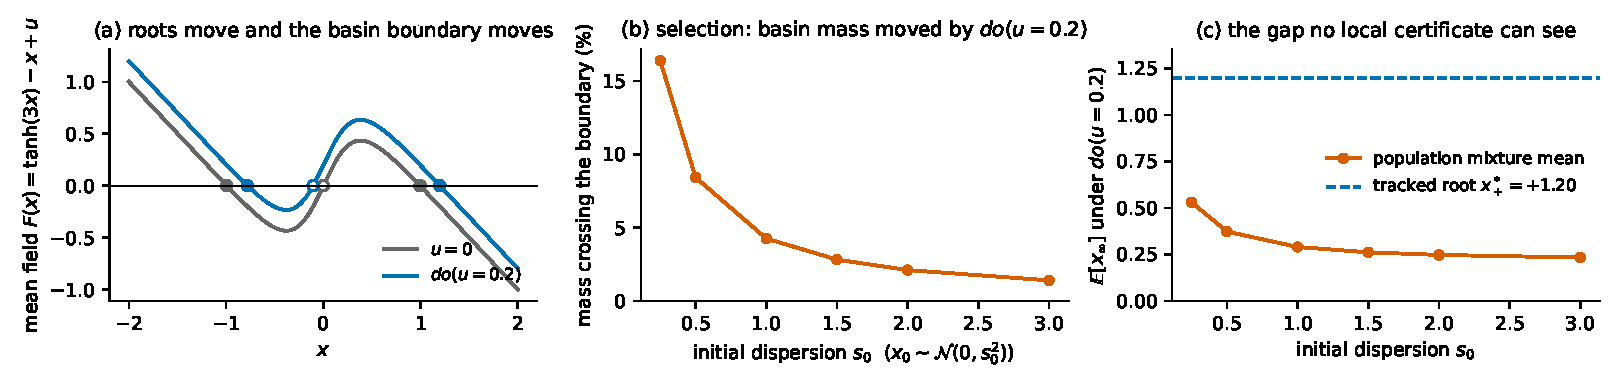
\includegraphics[width=0.9\textwidth]{figs/fig_e7.pdf}
\caption{E7. (a) Bistable mean field: under $\doop(u{=}0.2)$ both stable roots move \emph{and}
the basin boundary moves ($0 \to -0.105$). (b) Ensemble mass crossing the boundary vs initial
dispersion $s_0$. (c) Population mixture mean vs the equilibrium-tracking prediction
$x_+^* = +1.199$: the gap persists at every dispersion.}
\label{fig:e7}
\end{figure}

The bistable mean field $F(x) = \tanh(3x) - x + u$ has two stable equilibria and one unstable
one. At $u = 0$ the stable roots $\pm 0.995$ carry margins $+0.969$ \emph{each}: both
basin-local T1$'$ certificates are \Cid, correctly. Under $\doop(u{=}0.2)$ the roots
move to $-0.782$ and $+1.199$ (margins $+0.892$, $+0.991$), the basin boundary moves to
$-0.105$, and a stochastic-approximation ensemble ($N = 10^5$, gain $0.05$, noise $0.1$,
$x_0 \sim \mathcal{N}(0, 1.5^2)$) re-partitions from $50.2/49.8$ to $47.4/52.6$: $2.8\%$ of the
population crosses the boundary. Equilibrium-tracking at the positive root predicts $+1.199$;
the realized mixture mean is $+0.261$ --- a gap of $0.938$ no basin-local certificate can see
(tracking the negative root gives $1.04$; the conclusion is root-invariant). This is
Theorem~\ref{thm:main}'s multiplicity branch, and the \citet{blom2019beyond} caveat,
\emph{measured}.

Because the basin masses depend on the (arbitrary) initial distribution, we report the whole
curve (Figure~\ref{fig:e7}b,c): as $s_0$ ranges over $0.25$--$3.0$ the crossing mass falls from
$16.4\%$ to $1.4\%$, while the gap to the tracked root persists at every dispersion
($0.67$--$0.97$) and is largest when the population starts concentrated near the old boundary
--- the near-indifference case. The selection effect is not an artifact of the initial-condition
choice; its \emph{size} is the curve. The multiplicity diagnostic this motivates --- all stable
$\sigma$-solutions plus ensemble basin masses --- is Table~\ref{tab:ladder}'s last row.

% ============================================================================
\section{Related work}\label{sec:related}
% ============================================================================

\paragraph{Cyclic SCMs and dynamical abstraction.} \looseness=-1 \citet{bongers2021foundations}
give cyclic SCMs their solution-function semantics; \citet{mooij2013ordinary} and \citet{rubenstein2017causal}
characterize when an SCM consistently abstracts a dynamical system at equilibrium, and
\citet{bongers2018causal} prove that equilibration commutes with intervention under convergence
conditions; \citet{blom2019beyond} prove the representational impossibility our multiplicity
branch operationalizes; \citet{iwasaki1994causality}, \citet{dash2005restructuring}, and
\citet{weinberger2023intervening} warn that equilibrated models mispredict interventions. Our
delta: not ``when does the SCM abstract the dynamics'' but ``when do the dynamics validate the
SCM's $\doop$,'' as an equivalence for expectations-based adaptive learning, with the
E-stability characterization and sharp gain threshold. \citet{white2009settable} extend Pearl's
model for optimization, equilibrium, and learning (framework-level prior art; our delta is
theorem-level). On the macro side, E-stability is due to
\citet{marcet1989convergence,evans2001learning}, applied to policy by \citet{bullard2002learning}
and connected to the Lucas critique by \citet{evans2006adaptive}: that literature has the
stability theory but no causal semantics, the cyclic-SCM literature the reverse; T1 is the
bridge.

\paragraph{Learning in games and econometrics of learning agents.} \looseness=-1 No-regret
convergence to CCE is classical \citep{foster1997calibrated,hart2000simple,cesabianchi2006prediction,fudenberg1998theory};
\citet{nekipelov2015econometrics} use it as an identifying assumption;
\citet{bergemann2022counterfactuals}, \citet{magnolfi2023estimation}, and
\citet{syrgkanis2017inference} compute LP identified sets over equilibrium polytopes;
\citet{kline2024counterfactual} set-identify counterfactual outcomes in empirical games with the
point-vs-set boundary driven by equilibrium selection, not dynamics; and measured regret appears
as a regulatory audit statistic in \citet{hartline2024regulation}. The nearest neighbors are
\citet{lomys2025estimation}: $\varepsilon$-CCE set estimators for learning populations, with
support-function LPs, duality, and counterfactual bounds. Four choices separate our certificate
from their estimator: $\varepsilon$ is the \emph{measured realized regret} of the actual
trajectory, with no behavioral or algorithm-class assumption (they inflate by assumed worst-case
algorithm-class rates, themselves noting that realized regrets concentrate better); containment
is carried directly to the \emph{intervened} game's polytope rather than re-solved from
identified primitives; the certificate \emph{abstains} when vacuous; and the duals are reported
as regret prices. In causal games, \citet{hammond2023reasoning} define pre/post-policy
interventions with set-valued answers quantified over the equilibrium set (including a
credal-bounds reading) and present mechanised games as relational cyclic causal models, a
semantic bridge we build on; \citet{mishra2024causal} characterise a sound-and-complete family
of primitive interventions. Absent from that line is the identification layer supplied here:
conditions for point/interval/vacuous answers, a finite-time route from \emph{measured play}
rather than a fully specified model, and bounds actually computed. Non-convergent learning is
classical \citep{sato2002chaos,mertikopoulos2018cycles,pangallo2019best}; we use it as the
\Cbd{} rung's test bed. Performative prediction \citep{perdomo2020performative} is the
single-learner cousin: performative stability is case~1's analogue, and case~3 has no analogue
there because a single learner suppresses equilibrium selection.

% ============================================================================
\section{Limitations and open problems}\label{sec:limitations}
% ============================================================================

\looseness=-1 \textbf{Exactness class.} T1 is exact for the linear class; T1$'$ is local and
requires hyperbolicity; the global nonlinear statement leans on Assumption~\ref{ass:R}, parts
of which are guarded at runtime rather than decided a priori --- typed degradation to \Cem{} is
the honest response, but a sharper decidable characterization for structured nonlinear classes
is open, as is a bifurcation-aware treatment of the refused boundary cases. \textbf{Game scale.} The CCE LP is exponential in the number of players;
sampled and relaxed bounds with certified gaps are the scale path. \textbf{Stage-game scope.}
The demarcation of which learning families escape the stage-game polytope
(Remark~\ref{rem:scope}) is companion work. \textbf{Economics-facing model.} E4 is a bespoke
static-timing toy; a standard-timing calibrated New-Keynesian exercise is required before policy
conclusions. \textbf{Diagnostics not yet shipped.} E7's basin masses are computed by the
experiment, not a shipped instrument, and E2's ``non-convergent'' label lacks a Lyapunov
estimate of the learning flow; both are cheap follow-ups.

% ============================================================================
\section{Conclusion}\label{sec:conclusion}
% ============================================================================

\looseness=-1 ``When can you trust an equilibrium counterfactual?'' has, for well-delimited
classes, a three-part answer a machine can check: \emph{trust it} exactly when the mean dynamics are
E-stable and the stable solution is globally unique; \emph{bound it} by the measured-regret CCE
interval when the system is a finite game, with no assumptions beyond the trajectory log;
\emph{and otherwise do not} --- but demand the diagnostics, for certified failure is usable
knowledge: the Lucas critique not as a slogan but as a computable property of an intervened
system, firing exactly where it should.

% jmlr.cls already sets \bibliographystyle{plainnat}.
\bibliography{references}

\clearpage
\appendix

% ============================================================================
\section{Proof of Theorem~\ref{thm:t1} (stochastic parts)}\label{app:t1}
% ============================================================================

Throughout, $e_k = x_k - x^*$ and $\nu_1, \dots, \nu_n$ are the eigenvalues of
$A \coloneqq B_{\doop} - I$ (so $\margin > 0$ iff $A$ is Hurwitz).

\paragraph{(2), noise bound.} With constant gain $\gamma$ and
$u_{\doop,k} = \E[u_{\doop}] + \xi_k$, where $\{\xi_k\}$ is a martingale-difference sequence
with $\sup_k \E[\|\xi_k\|^2 \mid \mathcal{F}_{k-1}] \leq \sigma^2$, the error recursion is
\[
e_{k+1} = M_\gamma e_k + \gamma \xi_k, \qquad M_\gamma = I + \gamma A .
\]
Let $\Sigma_k = \E[e_k e_k^\top]$. Then
$\Sigma_{k+1} = M_\gamma \Sigma_k M_\gamma^\top + \gamma^2 \E[\xi_k \xi_k^\top]$, and for
$\gamma < \gstar$ we have $\rho(M_\gamma) < 1$, so $\Sigma_k$ converges to the unique solution
$\Sigma_\infty(\gamma)$ of the discrete Lyapunov equation
$\Sigma = M_\gamma \Sigma M_\gamma^\top + \gamma^2 \Sigma_\xi$ with
$\|\Sigma_\xi\| \le \sigma^2$, namely
$\Sigma_\infty(\gamma) = \sum_{j \geq 0} \gamma^2 M_\gamma^j \Sigma_\xi (M_\gamma^\top)^j$.
Choose a norm in which $\|M_\gamma\| \leq 1 - c\gamma$ for some $c > 0$ depending only on the
spectrum of $A$ (possible for all $\gamma \le \bar\gamma < \gstar$ since
$\rho(M_\gamma)^2 \le 1 - 2\gamma\,c_0 + \gamma^2 c_1$ with
$c_0 = \min_i(-\operatorname{Re}\nu_i) > 0$). Then
$\|\Sigma_\infty(\gamma)\| \leq \gamma^2 \sigma^2 \sum_j (1 - c\gamma)^{2j}
\leq \gamma^2 \sigma^2 / (2c\gamma - c^2\gamma^2) = O(\gamma)$,
which is the claim $\limsup_k \E\|e_k\|^2 = O(\gamma)$.

\paragraph{(1) $\Rightarrow$ (3).} For decreasing gains satisfying $\sum \gamma_k = \infty$,
$\sum \gamma_k^2 < \infty$, the recursion \eqref{eq:sa} is a Robbins--Monro scheme whose mean
ODE is $\dot{e} = A e$. For linear $A$ Hurwitz, $x^*$ is the globally asymptotically stable
equilibrium of the mean ODE; the iterates are bounded almost surely (the quadratic Lyapunov
function $V(e) = e^\top P e$ with $A^\top P + P A = -I$ yields a supermartingale argument
standard for linear SA; see \citealp[Ch.~5]{kushner2003stochastic} or
\citealp[Ch.~3]{borkar2008stochastic}), and the ODE-method limit-set theorem
\citep{ljung1977analysis,benaim1999dynamics,kushner2003stochastic} gives
$x_k \to x^*$ a.s.

\paragraph{(3) $\Rightarrow$ (1) and the converse claim.} Suppose $\margin < 0$, i.e.\ some
$\operatorname{Re}\nu_i > 0$; by hyperbolicity we may assume no eigenvalue has zero real part
(the boundary case is refused by the instruments, Table~\ref{tab:ladder}). Then $x^*$ is a
linearly unstable zero of the mean field. Under the excitation condition (A4) of
Appendix~\ref{app:t1prime} (nondegenerate noise in the unstable directions) and gains
$\gamma_k = \Theta(k^{-\alpha})$, $\alpha \in (1/2, 1]$, the nonconvergence theorem of
\citet{pemantle1990nonconvergence} (repeller case) and \citet{brandiere1996algorithmes}
(saddle/``trap'' case) yields $\Prob(x_k \to x^*) = 0$. Hence (3) fails, and contrapositively
(3) $\Rightarrow$ (1). For the constant-gain converse, Lemma~\ref{lem:gain} gives
$|1 + \gamma\nu_i| > 1$ for every $\gamma > 0$, so the mean iteration diverges for every initial
condition with a nonzero component in the corresponding invariant subspace --- all but a proper
(measure-zero) subspace. \hfill\BlackBox

% ============================================================================
\section{Assumptions and proof of Theorem~\ref{thm:t1prime}}\label{app:t1prime}
% ============================================================================

\paragraph{Assumptions.}
\begin{enumerate}
\item[(A1)] $f \in C^1$ on an open set containing $x^*$; $F = f - \mathrm{id}$; $x^*$ is a
hyperbolic zero of $F$: $J = DF(x^*)$ has no eigenvalue on the imaginary axis. $DF$ is locally
Lipschitz at $x^*$.
\item[(A2)] $x_{k+1} = x_k + \gamma_{k+1}(F(x_k) + M_{k+1})$ with $\{M_k\}$ a
martingale-difference sequence with respect to a filtration $\{\mathcal{F}_k\}$:
$\E[M_{k+1} \mid \mathcal{F}_k] = 0$ and
$\E[\|M_{k+1}\|^2 \mid \mathcal{F}_k] \leq \sigma^2 (1 + \|x_k\|^2)$ a.s.
\item[(A3)] Gains: either constant $\gamma_k \equiv \gamma$, or decreasing with
$\sum_k \gamma_k = \infty$ and $\sum_k \gamma_k^2 < \infty$.
\item[(A4)] (For part (ii) only.) There exist $b, \delta > 0$ such that on
$\{\|x_k - x^*\| \leq \delta\}$,
$\E[\langle M_{k+1}, v \rangle^+ \mid \mathcal{F}_k] \geq b$ for every unit vector $v$, the
noise is a.s.\ bounded on that event, and $\gamma_k = \Theta(k^{-\alpha})$ with
$\alpha \in (1/2, 1]$.
\end{enumerate}

\paragraph{Part (i), constant gain (deterministic core).} The damped map is
$T_\gamma(x) = x + \gamma F(x)$ with $DT_\gamma(x^*) = I + \gamma J$. By Lemma~\ref{lem:gain}
applied to the eigenvalues of $J$, $\rho(I + \gamma J) < 1$ for every
$\gamma \in (0, \gstar(J))$. Pick a norm with $\|I + \gamma J\| \leq 1 - c\gamma < 1$; by (A1)
there is a ball $\mathcal{B}$ around $x^*$ on which
$\|T_\gamma(x) - x^* \| \leq (1 - c\gamma/2)\|x - x^*\|$, giving local exponential stability
with basin at least $\mathcal{B}$. With noise, the argument of Appendix~\ref{app:t1} applied to
the linearization, plus a standard perturbation bound for the locally Lipschitz remainder
\citep[Ch.~9]{benveniste1990adaptive}, yields
$\limsup_k \E[\|x_k - x^*\|^2 \mathbf{1}_{\{x_j \in \mathcal{B}\ \forall j \le k\}}] = O(\gamma)$:
iterates that remain in the basin concentrate at the mean-square $O(\gamma)$ scale.

\paragraph{Part (i), decreasing gain.} $J$ Hurwitz makes $x^*$ a (locally) asymptotically stable
equilibrium of $\dot{x} = F(x)$ with domain of attraction $\mathcal{D}$. Let
$K \subset \mathcal{D}$ be compact. On the event
$\Omega_K = \{x_k \in K \text{ for all large } k\}$, the SA limit-set theorem
(\citealp[Thm.~5.2.1]{kushner2003stochastic}; \citealp{benaim1999dynamics};
\citealp[Ch.~2]{borkar2008stochastic}) applies: under (A1)--(A3) the interpolated iterate
trajectory is almost surely an asymptotic pseudotrajectory of the mean flow, whose limit set on
$\Omega_K$ is a compact, invariant, internally chain-transitive subset of $K$; since the only
such subset of a compact set contained in the basin of a hyperbolic attractor is $\{x^*\}$
itself, $x_k \to x^*$ a.s.\ on $\Omega_K$. This is the precise sense of ``locally, on the basin
of $x^*$'': the theorem conditions on remaining in a compact subset of the basin, and
Section~\ref{sec:e7} is the measured demonstration of why the conditioning cannot be dropped
when multiple attractors exist.

\paragraph{Part (ii).} $x^*$ hyperbolic with an unstable eigenvalue is a repeller or a saddle of
the mean flow. Under (A2)--(A4), \citet{pemantle1990nonconvergence} (repellers) and
\citet{brandiere1996algorithmes} (saddles; see also \citealp{benaim1999dynamics}) give
$\Prob(x_k \to x^*) = 0$. The excitation condition (A4) is what rules out the degenerate case of
noise supported on the stable manifold; it is satisfied, e.g., by any noise with a density
bounded below on a neighborhood of the origin, and in particular by the Gaussian noise used in
Section~\ref{sec:e7}. \hfill\BlackBox

% ============================================================================
\section{Proofs for Section~\ref{sec:t2}}\label{app:t2}
% ============================================================================

\paragraph{Corollary~\ref{cor:asymptotic}.} The feasible set $\CCE_\varepsilon(G_{\doop})$ is a
polytope $\{\mu \geq 0,\ \mathbf{1}^\top \mu = 1,\ G\mu \leq \varepsilon\}$ whose constraint
matrix is fixed. It is nonempty for every $\varepsilon \geq 0$: any Nash equilibrium of the
finite game $G_{\doop}$ --- which exists --- lies in $\CCE_0$, and the set only grows with
$\varepsilon$. The optimal value of a bounded feasible LP is a piecewise-linear, hence locally
Lipschitz, function of the constraint right-hand side, with one-sided derivatives given by the
optimal dual multipliers (standard LP sensitivity). If $\varepsilon_T \to 0$, any weak limit
$\mu_\infty$ of $\{\mu_T\}$ satisfies $G\mu_\infty \leq 0$ by continuity of
$\mu \mapsto G\mu$ on the simplex, so $\mu_\infty \in \CCE_0(G_{\doop})$, and the LP values at
$\varepsilon_T$ converge to the values at $0$ by the Lipschitz property. \hfill\BlackBox

\paragraph{Corollary~\ref{cor:degeneracy}.} If $h$ is constant over $\CCE_0$, the interval
is a point and contains the limit of $\E_{\mu_T}[h]$ for any no-regret population by
Corollary~\ref{cor:asymptotic}. Conversely, if $h$ is non-constant over $\CCE_0$, pick
$\mu \in \CCE_0$ with $\E_\mu[h]$ different from the equilibrium point prediction; a
population playing i.i.d.\ draws from $\mu$ is no-regret (its realized regrets converge to the
nonpositive expected deviation gains) and its time-average converges to $\E_\mu[h]$.
Zero-sum example: for any $\mu \in \CCE_0$ of a two-player zero-sum game, the no-deviation
constraints give $\E_\mu[u_1] \geq \max_{a_1'} \E_\mu[u_1(a_1', s_2)] \geq v$ and symmetrically
$\E_\mu[u_1] \leq v$, so every CCE achieves the value $v$. \hfill\BlackBox

\paragraph{Corollary~\ref{cor:duals}.} Parametric LP: the max-side value
$V(\varepsilon) = \max\{c^\top \mu : \mu \in \CCE_\varepsilon\}$ is concave and piecewise-linear
in the constraint right-hand side (standard RHS-perturbation concavity of a maximization LP),
and nondecreasing because relaxing constraints can only increase the value. Along the uniform
inflation direction $\varepsilon = \varepsilon_0 + t\mathbf{1}$, at any $t$ where the optimal
dual is unique the derivative is $\sum_j y_j^*$, the sum of the optimal dual multipliers on the
inflated constraints; at kinks the one-sided derivatives are the extreme values of that sum over
the optimal dual face. The min side is the max side of $-h$, hence convex with the symmetric
statement. \hfill\BlackBox

\begin{remark}
Our LP solver returns the dual vector alongside the primal optimum, and the shipped
certificates carry $\{\partial\text{lower}, \partial\text{upper}, \partial\text{width}\}$ at the
measured $\varepsilon_T$. All experimental LP values in this paper are additionally verified by
independent weak-duality certificates: a dual-feasible $y \geq 0$ with
$(G^\top y)_j \geq v - c_j$ for all $j$ certifies that no feasible $\mu$ exceeds $v$, with slack
$\sim 10^{-14}$ in all reported cases.
\end{remark}

% ============================================================================
\section{Proof details for Theorem~\ref{thm:main}}\label{app:main}
% ============================================================================

\paragraph{Exhaustiveness.} Fix the class. (a)/(b): by (R1) the intervened mean field has
finitely many zeros, each hyperbolic, so each is either stable ($\margin > 0$) or unstable
($\margin < 0$); the number of stable zeros is $0$, $1$, or $\geq 2$. If (R2)/(R3) fail at
runtime (divergence, cycles, positive Lyapunov estimate), case~3 fires by its second clause.
(c): the LP width is a number; it is either $\leq$ tol (case~1(ii)) or $>$ tol, and in the
latter case the measured-$\varepsilon_T$ interval is either informative (case~2) or vacuous
(case~3). Every system in the stated classes therefore lands in some case.

\paragraph{Exclusivity.} Case~1(i) requires a globally unique stable $\sigma$-solution, which
the multiplicity clause of case~3 negates; case~1(ii) and case~2 split on width $\leq$ tol
versus $>$ tol; the remaining clauses of case~3 (all-unstable, (R)-failure, vacuity) each
contradict the preconditions of cases~1 and~2 directly.

\paragraph{Warrant.} Case~1(i): in class (a), Theorem~\ref{thm:t1} gives global convergence for
every $\gamma \in (0,\gstar)$ and a.s.\ convergence under decreasing gain --- globality is free
because the mean dynamics are linear. In class (b), let $x^*$ be the unique stable zero. By
(R2) the iterates a.s.\ remain in a compact set $K$; by the limit-set theorem the a.s.\ limit
set is an internally chain-transitive subset of the flow restricted to $K$, which by (R3) is a
subset of the zero set. By Theorem~\ref{thm:t1prime}(ii) (whose excitation condition we adopt
here) the unstable zeros attract with probability zero, so the limit set is a.s.\ $\{x^*\}$.
Case~1(ii) is Corollary~\ref{cor:degeneracy}; case~2 is Theorem~\ref{thm:t2} plus
Corollary~\ref{cor:duals}; case~3's clauses carry, respectively, the divergence certificate of
Theorem~\ref{thm:t1}'s converse, the runtime diagnostics, the abstention rule of
Remark~\ref{rem:width}, and the basin-local certificates plus the representational
impossibility of \citet{blom2019beyond} for the multiplicity clause.

\paragraph{Decidability scope.} In class (a) every condition is a spectral or LP computation.
In class (b) the theorem is decidable \emph{given} the enumeration of zeros (available by
bisection for the scalar systems used here, and by homotopy or interval methods more
generally); (R2)--(R3) are guarded, not decided --- the honest scope stated in
Assumption~\ref{ass:R}. In class (c) both conditions are single LP solves. \hfill\BlackBox

% ============================================================================
\section{Experimental details and reproducibility}\label{app:exp}
% ============================================================================

All experiments are single-file scripts against the released instruments; seeds are fixed
in-script; every number in Section~\ref{sec:experiments} is pasted from an actual run. LP values
carry independent weak-duality verification (Appendix~\ref{app:t2}). The instruments --- one per
row of Table~\ref{tab:ladder}: the equilibrium-vs-unrolling comparator, the spectral diagnostics
(stability margin and maximal stable learning rate), and the game instruments (CCE-polytope
constructor, LP bounds, measured realized regret, certifier) --- and the experiment scripts are
provided as an anonymized code artifact accompanying the submission; their public API
identifiers are redacted from this draft for double-blind review.

\paragraph{E1 (cobweb).} Demand $D(p) = 10 - p$, supply intercept $c = 1$, tax
$\doop(\tau{=}1)$ entering as the supply-intercept shift; SCM
$p = -(s/d)\,p^e + (a - c + s\tau)/d$, $p^e = p$. Regimes: A $s/d = 0.5$; B $s/d = 1.5$ (naive,
then damped $\gamma = 0.4 = \gstar/2$); C trend-extrapolating demand $b = 1.2$; D
$\arctan$ supply (scale $2.2$, steepness $12$) under adaptive expectations
$p^e{}' = (1-g)p^e + g\,f(p^e)$, with the chaotic gain $g = 0.14$ found by a Lyapunov scan over
$g \in [0.08, 0.52]$ and the largest Lyapunov exponent $+0.222$ computed over $8{,}000$ steps.
The linearized certificate at $p^*$ hedges at $\gstar = 0.073 < g$. Honesty note (regime D): the
\emph{time-averaged} price ($5.8747$) happens to sit near $p^*$ ($5.9562$) because the chaotic
attractor is roughly symmetric around the fixed point; the pointwise prediction fails completely
(the trajectory never settles), and the certificate hedges exactly there.

\paragraph{E2 (perturbed RPS).} Payoffs as in \citet{sato2002chaos} with
$\epsilon_X = 0.5$, $\epsilon_Y = -0.1$; intervention: payoff tax $0.3$ on $X$'s action $0$
(the intervened game built explicitly). Hedge (multiplicative-weights) population,
$T = 200{,}000$ rounds, seed $7$. Exact CCE interval for $X$'s payoff $[0.0667, 0.3091]$;
measured-$\varepsilon_T$ interval $[0.0646, 0.3120]$ at $\varepsilon_T = 0.0021$.

\paragraph{E4 (macro loop).} $\beta = 0.99$, $\sigma = 1$, $\kappa = 0.3$, demand shock
$\doop(u{=}{+}1)$; $T(\varphi) = (\beta + \kappa\sigma)/(1 + \kappa\sigma\varphi)$; cyclic SCM
$B = [[0, T], [1, 0]]$ closed by naive expectations; comparator horizon $2{,}000$, tolerance
$10^{-6}$; learning paths are the naive-expectations recursion (thirty steps shown).
$\varphi = 1.5$: $\margin = +0.057$, gap $7 \times 10^{-15}$, $\pi^* = +9.06$, $\pi_{30} = +8.79$.
$\varphi = 0.5$: $\margin = -0.059$, $\gstar = 0$, $\pi^* = -8.21$, $\pi_{30} = +249.6$.

\paragraph{E7 (bistable selection).} $F(x) = \tanh(3x) - x + u$; roots by bisection on a grid of
$6 \times 10^5$ points over $[-3, 3]$; margins $= -F'(\text{root})$. SA ensemble:
$N = 10^5$ learners, constant gain $0.05$, additive Gaussian noise (s.d.\ $0.1$), $4{,}000$
steps, $x_0 \sim \mathcal{N}(0, s_0^2)$, seed $0$; dispersion curve over
$s_0 \in \{0.25, 0.5, 1.0, 1.5, 2.0, 3.0\}$. Figures regenerated deterministically by the
released figure script from the same code paths and seeds.

\end{document}
